\documentclass[comsoc,conference]{IEEEtran}
\IEEEoverridecommandlockouts
\usepackage{cite}
\usepackage{url}
\usepackage{amsmath,amssymb,amsfonts}
\usepackage{algorithmic}
\usepackage{graphicx}
\usepackage{natbib}
\usepackage{textcomp}
\usepackage{xcolor}
\usepackage{tabularx,booktabs}
\usepackage{caption}
\usepackage{subfig}
\captionsetup[table]{name=Table, labelfont=bf, labelsep=period, font=small}
\captionsetup[figure]{name=Figure, labelfont=bf, labelsep=period, font=small}
\newcolumntype{C}{>{\centering\arraybackslash}X}
\setlength{\extrarowheight}{1pt}
\def\BibTeX{{\rm B\kern-.05em{\sc i\kern-.025em b}\kern-.08em
    T\kern-.1667em\lower.7ex\hbox{E}\kern-.125emX}}
\begin{document}

\title{Aspect-based Sentiment Analysis
	\\ \large{Track: T1-02 (A Hierarchical Model of Reviews for Aspect-based Sentiment Analysis)
	\\ Team: Naive Baes}
}

\author{
	\IEEEauthorblockN{Ijaz, Ramsha}
	\IEEEauthorblockA{ramsha.ijaz@mail.mcgill.ca}
	260665762
	\and
	\IEEEauthorblockN{Rahman, Aanika}
	\IEEEauthorblockA{aanika.rahman@mail.mcgill.ca}
	260662187
	\and
	\IEEEauthorblockN{Seol, Yunheum}
	\IEEEauthorblockA{yunheum.seol@mail.mcgill.ca}
	260677676
}

\maketitle

%\begin{abstract}\end{abstract}

\section{Introduction}

Sentiment analysis has been the technique used to mine opinions from customer reviews. The classical approach to this was to treat an entire sentence as a document and extract sentiments ("positive", "neutral", and "negative") based on all words. However, it has apparent limits for sentences that contain more than one aspect with conflicting sentiments. An example for this would be a review for a restaurant that says, "The food was tasty, but I don't think it came at a reasonable price". The sentence contains two aspects (i.e. \texttt{FOOD\#QUALITY}, \texttt{FOOD\#PRICES}) and two contradicting sentiments. Aspect-based sentiment analysis (ABSA) addresses this issue by classifying sentiments for a given aspect label.

ABSA has its own issue where it analyzes each sentence in a review independently, not taking into account the argumentative structure of the review. The paper "A Hierarchical Model of Reviews for Aspect-based Sentiment Analysis" \cite{T1-P2}, implements improved versions of Long Short-Term Memory (LSTM) to address this problem. The resulting hierarchical LSTM (H-LSTM) yields better accuracy than their sentence-level baselines. While the H-LSTM performance is noteworthy for certain languages, mentioned competing models perform better for the English dataset. 

We are tasked with recreating and improving the baselines reported in our paper of interest, as well as exploring simple Machine Learning algorithms wither lesser computational complexity. The paper considers datasets of customer reviews in 5 domains and 8 languages, with a total of 11 domain-language datasets. Given the time frame and our objective, focus will be placed on only the English datasets, which consist of two domains, restaurants (REST) and laptops (LAPT).

\subsection{Hypotheses}

Classical machine learning algorithms fail to model long-term dependencies of words in a sequence, which are better addressed by LSTMs. Nevertheless, we expect that with appropriate representation and hyperparameter tuning, simple models can yield better results than the results of the baseline (i.e. LSTM) in the paper but not the improved model in the paper (i.e. H-LSTM). Among such models, we anticipate Logistic Regression and Support Vector Machine (SVM) to be the strongest candidates. After reproducing the baseline in the paper, the LSTM can be further improved by adding deep layers. 

\section{Preprocessing}

\subsection{Data Analysis}

% no. polarities, no. reviews, no. sentences, no. sentence-aspect pairs (recall size of dataset can influence what models are best)
Each sentence in each dataset has zero to multiple associated aspects, where each aspect is composed of an entity and attribute (e.g. \texttt{FOOD\#QUALITY}), and is assigned one of three polarities (i.e. positive, neutral, negative) to describe sentiment. While there are 400-550 reviews and 2200-2600 unique sentences per dataset, following the paper, sentences with two aspects are made to occur twice, once with each aspect and sentences with no aspects to be ignored. This results in 3432 and 3774 sentence-aspect pairs as data samples for the REST and LAPT datasets respectively.

% no. categories/aspects (no. entities, no. attributes), distribution of sentences among aspects (influence threshold for aspects tested)
There are 12 and 88 potential aspect categories for REST and LAPT datasets respectively. Since the LAPT dataset has an overwhelming number of aspect categories, a threshold was set when encoding aspects such that aspects with a lower frequency are categorized under "miscellaneous", resulting in 12-15 encoded aspects per dataset.

% distribution of sentences among polarities, distribution of sentences w/ one aspect, w/ many aspects w/ same polarity, w/ many aspects w/ different polarities
As shown by the distribution of sentence-aspect pairs among polarities in Figure~\ref{P1}, the majority have a positive polarity and there are not many samples with a neutral polarity. Furthermore, only 10-15\% of sentences have associated aspects with differing polarities, as noted in Figure~\ref{P1}. Given that almost 90\% of our data have consistent polarities despite aspect, predicting polarity despite aspect per sentence may not result in poor results. 

\begin{figure}[!htb]
    \centering
  \subfloat[\label{a}]{%
       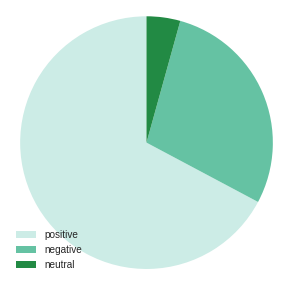
\includegraphics[width=0.45\linewidth]{images/anal_pol_REST.png}}
    \hfill
  \subfloat[\label{b}]{%
        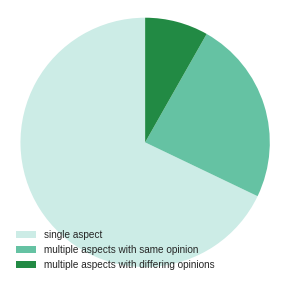
\includegraphics[width=0.45\linewidth]{images/anal_asp-pol_REST.png}}
    \\
  \subfloat[\label{c}]{%
        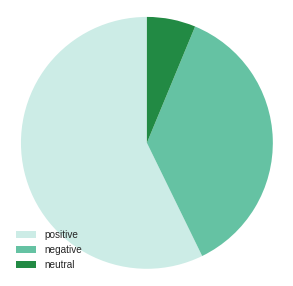
\includegraphics[width=0.45\linewidth]{images/anal_pol_LAPT.png}}
    \hfill
  \subfloat[\label{d}]{%
        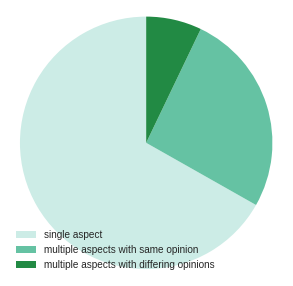
\includegraphics[width=0.45\linewidth]{images/anal_asp-pol_LAPT.png}}
  \caption{(a), (c) Distribution of sentence-aspect pairs among polarities (b), (d) Distribution of sentences with the same/differing polarities for REST, LAPT datasets respectively}
  \label{P1} 
\end{figure}

\begin{figure}[!hb]
    \centering
  \subfloat[\label{a}]{%
       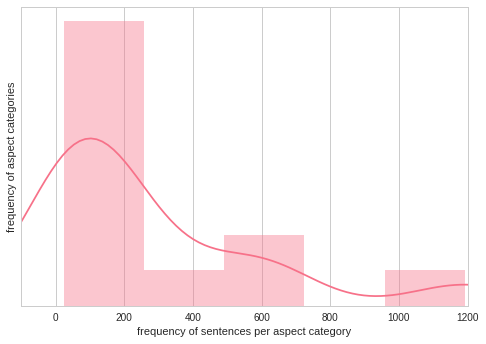
\includegraphics[width=0.9\linewidth]{images/anal_asp-freq_REST.png}}
    \hfill
    \\
  \subfloat[\label{c}]{%
        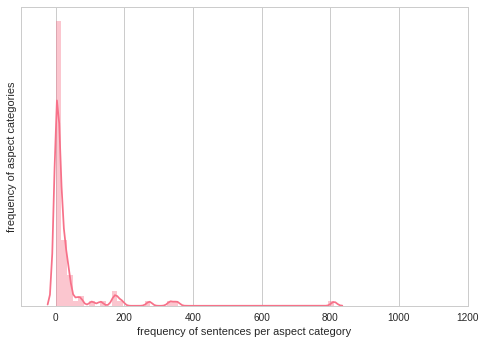
\includegraphics[width=0.9\linewidth]{images/anal_asp-freq_LAPT.png}}
    \hfill
  \caption{(a), (b) Distribution of aspect categories for REST, LAPT datasets respectively}
  \label{P2} 
\end{figure}

\subsection{Data Cleaning}

% remove punctuation, remove numbers, convert to lowercase
For each sentence and target word, we eliminate all non-word and non-space characters (e.g. punctuation, numbers, symbols) and convert all letters to lowercase. This avoids having multiple variations of the same word in our vocabulary when vectorizing our data. For instance, when calculating the word count, 'Amazing!' and 'amazing' will be taken as different words otherwise.

% remove stop words, lemmatize, avoid stemming
We lemmatize certain words (i.e. group together different inflections of the same word). By noting the "part of speech"  (POS) tag of a word using the \texttt{TextBlob} library, only nouns, verbs, adjectives and adverbs are lemmatized so that words like 'us' are not converted to 'u'. Note that lemmatization is more effective than stemming as it converts the word into its root word, rather than stripping the suffices. For example, 'was' and 'being', with root word 'be', will not be considered to have the same meaning otherwise. Taken from the \texttt{nltk} library, stop words (e.g. pronouns, prepositions, conjunctions) are further removed before vectorizing our data. High frequencies of stop words that have no value (e.g. 'the') and having different inflections of the same word (e.g. 'eating' and 'eat') may distort what words are perceived valuable by a model.

% avoid spellcheck as problematic
As observed when implementing a spell check, there is a chance of correcting words to an unintended word, which may unfavorably influence the polarity predicted by the model. Hence, a spell check was disregarded.

\subsection{Data Representation}

Global Vectors for Word Representation (GloVe) \cite{GloVe} is a method of obtaining pre-trained embeddings, where word vectors capture meaning in vector space and takes advantage of global count statistics instead of only local information. Following the paper of interest, we use pre-trained GloVe embeddings, to first reproduce the same baseline performance for our Neural Network models. To factor in the aspects as part of the input, both the entity and attribute of an aspect are converted into their the respective word embeddings with the help of GloVe embedding matrix, which are then averaged to obtain the final aspect embedding.

Looking at sentence representation, we then use average perceptron tagger from the \texttt{nltk} library to attach a POS tag to each word. \texttt{nltk.help.upenn\_tagset()} command returns all possible labels for POS, and it is what was used throughout the report. We further carry out IOB2 (Inside-Out-Beginning) tagging for each word to reflect the sentimental and grammatical structure of a review sentence. 

While attempt to reproduce the data representation in the paper of interest was made for the neural network models, we use bag-of-word representations for all classical algorithms to be implemented (e.g. Decision Tree, Random Forest, and SVMs) given limited time and hands on the project. Note that this only takes advantage of local information. Hence, we derive vector representations for each sentence, where each unique word in the training set is used a feature to result in one of three following options:
\begin{itemize}
    \item Binary Bag-of-Words (BBoW): binary values indicating the presence of each unique word;
    \item Frequency Bag-of-Words (FBoW): integer values representing the frequency of each unique word;
    \item Term Frequency-Inverse Document Frequency (TF-IDF): weight values that encode the relative importance of a word in an abstract.
\end{itemize}
To represent the aspect in our input, we first encode our aspect as a binary vector $v \in \mathbb{F}_2^n$ where n=12 for the REST dataset, and n=15 for the LAPT dataset\footnote{For the sake of efficiency and brevity, we decrease the number of categories to 15, by categorizing all categories after the 14th as miscellaneous}. Then we concatenate this aspect vector to the original Bag-of-Word representation. In preliminary experimenting, this concatenation as opposed to naive sentiment sentiment analysis without aspect taken as input, generally underfit for the training yet demonstrates an improved level of performance for both the validation and test set.

Further additional preprocessing measures such as trimming words or lemmatization seems to penalize against the models where aspects are not taken as input, but it aids models where aspects are taken as features. This is a better result for us since our main focus here is to show the importance of Aspect-Based sentimental analysis. However, one can conclude that this might be heavily dependent on the number of aspects one is given as input for a model.

\section{Algorithm Selection and Implementation}

After converting the \texttt{xml} file to the desired format and working through the preprocessing pipeline as explained above, the datasets are split into training, validation and test sets with ratio 6:2:2 and converted into representations mentioned earlier. Where the training validation sets were used to select optimal parameters, the test set was left out and used to evaluate the performance of the best model from each classifier. Following the paper\footnote{Although not explicitly mentioned by the paper, this was confirmed by the author via email}, accuracy is reported as our evaluation metric. % Accuracy can be computed as follows: \textbf{accuracy} = \frac{\textbf{TP}+\textbf{TN}}{\textbf{TP}+\textbf{FP}+\textbf{FN}+\textbf{TN}} where TP...

We see the standard LSTM and CNN used in the paper as the baselines to overcome. However, we only focus on reproducing and improving the LSTM since the paper did not specify how the CNN has been fit, trained and tuned. Therefore, for all neural network models implemented, we adopt one layer per input (i.e. one for the sentence and another for the aspect) and combined them at another hidden layer with possibly more hidden layers added.

Simple baselines can also perform better than complex models if properly tuned and are therefore explored as well. Hence we explore many as mentioned below, by using their respective implementations from \texttt{sci-kit} \texttt{learn}. 

\subsection{Naive Bayes}

As a supervised learning model using generative methods, Naive Bayes explicitly models the joint probability and then uses the Bayes rule to compute the posterior conditional probability $P(y|x)$ as follows:
\begin{flalign}
P(y|x_1,...,x_n) = \frac{P(y)P(x_1,...,x_n|y)}{P(x_1,...,x_n)} = \frac{P(y)P(x|y)}{P(x)}
\end{flalign}
where $y$ is a given class variable and $x_1,...,x_n$ are features forming the feature vector $x$.

As the name suggests, it is a \textit{naive} prediction of the data as it assumes that the effect of the value of a predictor $x_i$ on a given class $y$ is independent of the values of other predictors, for some $i=\{1,...,n\}$. This assumption is called class conditional independence. If feature independence and linearity of the data is violated, the Naive Bayes classifier would be assumed to perform poorly as semantic context of specific words used in conjunction with one another may be lost.

We chose to implement Naive Bayes as one of our simple classifiers since it is very time efficient and suitable for high-dimensional datasets, and hence a useful starting point. Moreover, when making decision regarding preprocessing (e.g. list of stop words, maximum number of features) based on the performance of the model, Naive Bayes is an excellent candidate to assess such decisions due to its efficiency. 

\subsection{Logistic Regression}

Logistic models, also known as logit models, are the most famous example of a generalized linear models, where response Y with input features $\mathbf{X}$ are assumed to have following relationship:
\[\ln\bigg(\frac{E[Y]}{1-E[Y]}\bigg) = \mathbb{X}W\]
This is assumed to be one of the strongest candidates since our response is grouped binary data with sparse matrices as input features.

\subsection{Linear Support Vector Machine}

Linear Support Vector Machine (commonly known as SVM) can be thought of as the "modern version" of historically famous perceptron algorithm. It fits a classifier that maximizes the margin between the data and the hyperplane separating different classes of data. Linear SVM yields a solution to the following optimization problem for the binary case (can be generalized to a multi class problem through one-versus-the-rest, one-versus-one and other schemes):
\[
argmin \frac{1}{n} \bigg(\sum_{i=1}^n max(0. 1-y_i(\vec{w}^T\vec{x_i}-b))\bigg) + \lambda||\vec{w}||^2
\]

SVM has higher speed and better performance with a limited number of samples. This makes the algorithm very suitable for text classification problems, where often dataset has a limited size. SVM can learn regardless of the dimension of the feature space. Therefore, with an appropriate kernel function it can work well even if the data is not linearly separable in the base feature space. On the contrary, a poorly chosen kernel will add onto the computational cost. 

Considering the fact that Linear SVM is able to classify linearly separable problems, we chose it as one of our baselines since text classification and sentiment analysis is essentially a linearly separable problem. Below is the graph of the accuracy measure obtained from a Linear SVM:

\subsection{Non-Linear Support Vector Machines}

Support vector machine classifier can be generalized to a problem that is not linearly separable, either by maximizing the soft margin, or by adopting a non-linear kernel function. Some common choices would be polynomial kernels, sigmoid kernel, and radial basis function, which is defined as:
\[
rbf(\vec{x}) = \exp{-\bigg(\frac{|\vec{x}-\vec{x}`|}{2\sigma^2}\bigg)}
\]
which is the kernel part of a typical Gaussian distribution.

We test out a non linear kernel, namely the radial basis function (rbf) and polynomial kernel functions to see whether this would bring a model with better performance. 

\subsection{Decision Trees}

Decision Trees works quite similar to the decision process of a human brain. Unlike other classifiers, it interprets the logic of the data that needs to be classified and outputs a decision based on the conclusion it has acquired from the interpretation. A Decision Tree is a tree where each node represents a feature, each branch represents a decision rule and each leaf represents an outcome for the decision rule implemented. \cite{DT1} The Decision Trees are able to handle continuous and categorical values and can generate understandable decision rules for the values entered. Thus, they are simple and fast as when performing classification of linearly separable data. On the hindsight, if the hyperparameters such as the \texttt{max\_depth} if not chosen appropriately, the tree becomes computationally expensive to train. 

We chose Decision Tree as a baseline classifier as it is faster and an efficient model that works well with linear problems such as text classification.

\subsection{Random Forests}

Random Forest is an ensemble model for Decision Trees as it essentially accumulates the Decision Trees and averages the information gain from all the trees during the classification process. Unlike a bagging model where all features are considered for splitting a node, Random Forest selects a subset of features at random out of the entire dataset and the best split feature from the subset is used to split each node in a tree. Hence, it works very well compared to a single Decision Tree. Random Forest are competitive in classifying multi-class text as multiple trees collectively extract features and classify the text according to the high gain from the dataset. Therefore, careful tuning of hyperparameters is necessary in order to prevent the the model from overfitting. 

Since Decision Trees tend to overfit, we also implement Random Forest as a progression from Decision Trees. This classifier decreases the variance by averaging out several trees prediction which in turn reduces overfitting. We disregard the extremely randomized tree classifiers since it is computationally expensive (i.e. it takes more than an hour to train one tree) and severely underfits.

\subsection{Long Short Term Memory (LSTM)}

LSTMs are a special type of recurrent neural networks that have achieved better results than standard recurrent neural networks for many of the tasks. Any type of RNNs can use parts of the past information to make a better estimate of the future information, and in principle is capable of addressing the long term dependencies between the sequential inputs. For example, if we were to extract the sentiment from a restaurant review that says "I had an issue with the price, yet the overall they served us great food...it could have been cheaper, still." given the aspect \text{FOOD\#PRICE}. The words \textit{price} and \textit{cheaper} are related, but they are apart by a collection of words. In practice RNNs fail to reflect this structure in their model, and LSTM has been devised as a solution to this. They also address the problem of vanishing/exploding gradient problem by adopting logic gates.

\subsection{Gated Recurrent Unit (GRU)}

Gated recurrent unit (GRU) is a type of recurrent neural network introduced in less than four years ago by Cho et al. It can be thought as a variation of LSTM, devised in order to address the vanishing gradient problem, an issue that commonly happens for vanilla and recurrent neural networks. What makes GRUs special from either standard recurrent neural networks or other improved methods such as LSTM is the use of update gate and reset gate. They are two vectors that play a critical role on deciding what information should be passed to the output layer. What stands out is that they can be trained to store information from the past, without washing through time or remove irrelevant information.

The update gate facilitates the model to determine what proportion of the information from the past needs to be fed along to the future. The rest gate, on the other hand, it determined how much proportion of the past information to forget. It is a powerful characteristic since it gives the model the ability to make decision to copy all the information from the past while eliminating the risk for vanishing gradient problem.

\section{Hyperparameter Exploration}

\begin{table}[!tb]
\begin{tabularx}{\linewidth}{@{}l*{1}{C}c@{}}
\toprule
Model & Considered Hyperparameters \& Ranges \\
\midrule
Naive Bayes & 'alpha': np.arange(0.01, 1.01, 0.01) \\
\midrule
Linear/Radial SVM, & 'C': np.logspace(-2, 2, num=8) \\
Logistic Regression & 'max\_iter': np.arange(10, 100, 10) \\
\midrule
Decision Trees, & 'max\_depth': np.arange(13, 17) \\
Random Forest & 'max\_features': np.arange(0.1, 0.5, 0.1) \\
\midrule
Random Forest & 'n\_estimators': np.arange(2, 12) \\
\midrule
GRU, LSTM & 'number of hidden layers': np.arange(5) \\
& 'number of hidden units': np.arange(35, 47) \\
& 'early\_stopping::patience': np.arange(2, 16) \\
& 'dropout': np.arange(0.1, 0.5, 0.1) \\
& 'recurrent\_dropout': np.arange(0.05, 0.2, 0.05) \\
& 'activation': ['sigmoid', 'ReLu', 'None', 'tanh'] \\
\bottomrule
\end{tabularx}
\caption{Hyperparameters tuned for all algorithms}
\label{M1}
\end{table}

The hyperparameters adjusted for simple algorithms and their respective ranges are mentioned in Table~\ref{M1}. Since the effect of tuning some hyperparameters was random or not significant, some were explored but removed from the final experiments as elaborated below.

\subsubsection{Laplace/Lidstone smoothing parameter $\alpha$}

Naive Bayes only has this hyperparameter, which is tuned to better handle features seen in the validation or test set but not in the training set. Without smoothing, features seen only in the training set would classify the corresponding sentence of the testing example as impossible and thus affect its classification. For all datasets and their respective data representations, validation accuracies were poor for low $\alpha$. Accuracies peaked mid range for the REST dataset, but at greater alpha for the LAPT dataset, with the exception of the TF-IDF representation. In the case of the LAPT dataset, this perhaps implies the presence of features in training set which is not present in the validation set and this also foreshadows the general possibility of other models performing poorly on the LAPT dataset. Since the TF-IDF representation minimizes this issues, too much smoothing in this case leads to bad classifiers, as classification accuracy approached that of a random classifier. 

\subsubsection{Penalty parameter C, maximum iterations}

Reducing the penalty parameter C gives the model a chance to learn the underlying pattern by allowing for misclassification of some points. In the case of Linear SVM, larger C will influence a smaller-margin hyperplane if that hyperplane does a better job of getting all the training points classified correctly. In our case, Linear SVM and Logistic Regression performs better with a smaller value C for all datasets and representations, while there does not appear to be a consistent pattern for Radial SVM. Although it appears as thought the effect of tuning maximum iterations is insignificant, in some cases the same penalty may results in a wide range of accuracies, fixing the optimal number of maximum iterations avoids low accuracies. This is particularly when the optimal penalty is low, as otherwise for higher penalties, the accuracies are more consistent.

\subsubsection{Tree hyperparameters}

Such hyperparameters includes maximum number of features to consider at each split, maximum depth, and number of estimators (trees) in the forest (n-estimators) in the case of the Random Forest classifier. While tuning max features and max depth does not largely influence accuracies for BBoW and FBoW representations, we have clearer observations for the TFIDF representation. In the case of the REST dataset, accuracies decrease as max features and max depth increase; whereas for the LAPT dataset, accuracies increase as max features increase, while max depth still plays an insignificant role. Looking at maximum depth, if there are many words in our vocabulary with high entropy, then allowing our trees to use more of those words will create a more accurate ensemble of trees, which is implied otherwise for the REST dataset in our case. The number of estimators in the forest has a similar rationale. Since results are averaged from the results of the trees, having more trees can reduce misclassifications that are caused by random feature selection. Since the effect of tuning minimum samples per leaf and split, and the criterion used for deciding the split at each level of the tree appears to be insignificant or random in most cases, they are ignored. 

The hyperparameters adjusted for the neural networks (i.e. GRUs, LSTMs) are number of hidden layers, number of hidden units in a hidden layer, regular and recurrent dropout rates, patience level for early stopping regularization, and activation function for the layers. The ranges considered are mentioned in Table~\ref{M1}. 

\subsubsection{Number of hidden layers}

The number of layers stacked can really offer a breakthrough to many prediction problems. As it has been pointed out, the success of deep neural networks is mainly attributed to the hierarchical structure introduced through having multiple layers. Even a sufficiently large Multi-Layer Perceptron with one hidden layer (or known as the "vanilla" neural networks) can approximate almost every function; however, adding depth to a network can offer a space-efficient alternative to adding a huge number of nodes to one hidden layer (Hermans and Schrauwen). Each layer added can be thought of as a machine that processes certain part of the task we aspire to find the solution of it, and passes it to the next one. If it helps, the whole network can be thought of as a group of factory workers on the same conveyor process, trying to assemble a car together. Each layer would be like a worker who does a specific, designated task, such as attaching the door to the car, putting the engine inside the car, or painting it. As the conveyor belt system has offered a significant improvement in the work environment, so do the deep neural networks with multiple hidden layers. For our case, GRU, RNN and bi-directional LSTM perform the best when the network has two hidden layers. 

% provide reference for (Hermans and Schrauwen)? 
%https://papers.nips.cc/paper/5166-training-and-analysing-deep-recurrent-neural-networks

\subsubsection{Number of hidden units in hidden layers}

Let us use the analogy between networks with multiple hidden layers and the group of works on a conveyor belt once again. In most cases, each worker on the belt is specialized at only few subtasks. Some of the tasks would need someone more competent, but others not necessarily. In our case, the number of hidden units can be thought as a way to set how specialized and competent one worker should be for a given task. GRU performs best when the number of hidden units is between 35 neurons and 42 neurons, peaking with 41. For our LSTM, the ideal number of hidden units is 41.

\subsubsection{Regular drop-out rate}

By definition, drop-out refers to ignoring neurons (or units) that are randomly selected during some stage of training process such that they will not be processed through the feed-forward stage or the backpropagation stage. In the mentioned analogy, if the efficiency rate of a factory suddenly dropped, a way to determine the part that slows done the entire system is by randomly removing or replacing some of the workers and assess the change in efficiency. As a more technical description, individual nodes are either kept with a probability of $p$ or dropped out of the network with a probability $q:= 1-p$. Surprisingly for our case it does not play a great role in terms of the fit, so we have kept it as 0.5. Unlike the recurrent drop out rate, it usually gets applied in either the input layer or the output layer.

%https://medium.com/@amarbudhiraja/https-medium-com-amarbudhiraja-learning-less-to-learn-better-dropout-in-deep-machine-learning-74334da4bfc5 

\subsubsection{Recurrent drop-out rate}

As suggested above, the recurrent drop out process drops the connection between the hidden layers. A way to visualize the difference between the two processes is shown in Figure~\ref{M2}. 

\begin{figure}[!htb]
\centering
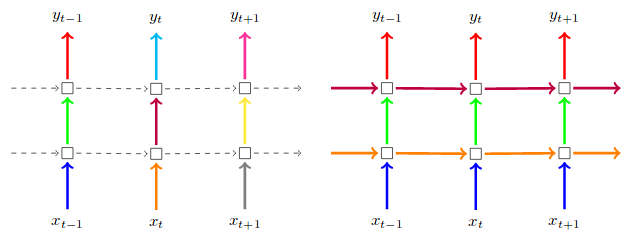
\includegraphics[scale=0.4]{images2/recurrent_drop_out_rate.png}
\caption{Visualization of recurrent drop-out rate}
\label{M2}
\end{figure}

The regular drop out drops the connection to or from input/output layers (i.e. vertical arrows) whereas the recurrent drop out drops the connections between hidden layers (the horizontal arrows). In our case, it performs the best at 0.2.

%https://arxiv.org/pdf/1512.05287.pdf

\subsubsection{Patience for Early Stopping}

Early stopping is a regularization process where the possibility of overfitting is reduced by the following procedure. The first step is to keep track of training and validation accuracy - or any other evaluation metric of choice - at each epoch. Then at the end of each epoch remark how the metric for the validation set changes; if it continuously decreases for a certain number of epoch, the learning process gets terminated early (hence the procedure is named so). The hyperparameter for this procedure would be the number of epoch to observe the decreasing trend of validation metric (or how many epochs we would "allow" to continue even if the validation metric decreases), or commonly known as the patience. Something to remark for our model is that as the magnitude of patience increases the model performed more poorly on the validation set for both the REST and LAPT dataset. Our hyperparameter tuning showed the models performed the best at patience of 2.

\subsubsection{Choice of activation function}

For any neural network the choice of activation function, particularly for hidden layers is crucial. The list of choices available to us to Rectified linear units, tanh, and sigmoid functions. After tuning we concluded that having ReLu function for hidden layers and sigmoid for the output layers give the best models.

For LSTM and GRU, the loss function used to evaluate the performance is categorical cross entropy supported from keras library, i.e. the loss function $J(\vec{w})$ would be as follows:
\[
J(\vec{\theta}) = - \sum_{n=1}^N\sum_{m=1}^M\{1\{y^{(n)}=k\}\log P(y^{(i)} = k|x^{(i)}; \theta)\}
\]
\noindent which is a multinomial generalization of the binary case
\[
J(\vec{w})- \frac{1}{N} [ \sum_{n=1}^N \{y^{(n)} \log \hat{y}^{(n)}(\vec{x}) + (1-y^{(i)})\log(1-\hat{y}^{(n)}(\vec{x})) \}]
\]
where we have 
\[
\hat{y}(\vec(x)) = \frac{1}{1+e^{\vec{w}^t\vec{x}}}
\]

In order to avoid overfitting, we have adopted early stopping with patience level of 2-16 as our regularization method. Another choice of ours is regular dropout with rate 0.5 with recurrent drop out with rate 0.2. The method of early stopping prevents overfitting in the sense that it stops the entire learning procedure once it starts learning the "unnecessary" traits from the training set, making sure that it will not go through situations where the model would overfit. Both of the drop out methods check the existence of a particular unit or neuron that has picked up the features/traits that are specific to the training set.

\section{Results \& Discussion}

\begin{table*}
\begin{tabularx}{\textwidth}{@{}l*{11}{C}c@{}}
\toprule
Domain (Representation) & CNN (paper) & LSTM (paper) & LSTM & GRU & Naive Bayes & Logistic Reg. & Linear SVM & Radial SVM & Decision Trees & Random Forest \\ 
\midrule
REST (GloVe)    & 82.10 & 81.40 & \textbf{90.76} & 88.57 & -     & -     & -     & -     & -     & -     \\
REST (BBoW)     & -     & -     & -              & -     & 79.88 & 79.59 & 80.03 & 72.89 & 73.62 & 77.26 \\
REST (FBoW)     & -     & -     & -              & -     & 80.76 & 80.47 & 78.72 & 72.45 & 72.89 & 78.57 \\
REST (TFIDF)    & -     & -     & -              & -     & 83.24 & 81.92 & 82.51 & 73.47 & 73.76 & 77.55 \\
LAPT (GloVe)        & 78.40 & 76.00 & \textbf{87.93} & 85.50 & -     & -     & -     & -     & -     & -     \\
LAPT (BBoW)         & -     & -     & -              & -     & 69.50 & 70.82 & 68.70 & 56.76 & 66.31 & 69.23 \\
LAPT (FBoW)         & -     & -     & -              & -     & 71.75 & 69.23 & 68.70 & 40.98 & 62.33 & 68.70 \\
LAPT (TFIDF)        & -     & -     & -              & -     & 73.87 & 69.23 & 72.68 & 57.29 & 61.14 & 65.52 \\
\bottomrule
\end{tabularx}
\caption{Test results for all classifiers, where the evaluation metric is accuracy (4 s.f.) and highest scores are bolded}
\label{R1}
\end{table*}

%Summary: table of results (accuracy metric), graphs (hyper-parameters, loss vs. epochs, etc), compare models, compare hyper-parameters, note an example which algorithms analyze a sentence difference (if possible), note what features of a model appears to bring up/down the performance
% ---
% compare models (simple classifiers)
% compare models (complex classifiers)
% compare models (overall)
% compare data representations (simple classifiers) i.e. BBoW, FBoW, TFIDF
% discuss data representation (complex classifiers) i.e. Glove
% compare datasets (simple classifiers) i.e. REST, LAPT
% compare datasets (complex classifiers) i.e. REST, LAPT

\subsection{Simple Classifiers}

Among simple classifiers, although Linear SVM has the best training accuracies as shown in Table~\ref{A1}, Naive Bayes and Logistic Regression have similar testing accuracies to Linear SVM, which simply suggests more overfitting for Linear SVM. The results suggest that provided the concatenated input features, these three algorithms perform decently, even to the point where it surpasses the evaluation metric of one of the baseline performances in the paper (i.e. LSTM) for the REST dataset. 

Despite poorer testing accuracies for the remaining simple classifiers, the difference between their training and testing accuracies are not large. The SVM with the non linear kernel surprisingly underperforms compared to its linear equivalent, suggesting the dataset might in fact be linearly separable. As expected the Random Forest classifier shows a better fit than Decision Trees. 

When comparing datasets for simple classifiers, we observe that the training accuracies are not widely different. However, since the difference between training and testing accuracies is greater for the LAPT dataset, there tends to be more overfitting on the LAPT dataset. Perhaps this is due to poor data representation or limited hyperparameter tuning for this particular dataset. This may require more comprehensive data analysis to make adjustments. 

Out of the classical ML algorithms, we remark on Naive Bayes, Linear SVM, Logistic Regression, and Random Forest.

\subsubsection{Naive Bayes}

Naive Bayes shows a huge improvement in performance since the additional preprocessing measure. The test accuracy shows more than 10 percent increase once the lemmatization applies. One question that might arise is the level of performance improvement is less pronounced for BBoW (there are a few entries with polarity "neutral" yet most of them are either "positive" or "negative".) It seems that the conditional independence assumption of response given the features describe our dataset well enough. It also outperformed the baselines if TF-IDF representation is used instead of mere bag-of-words.

\subsubsection{Random Forest}

Preprocessing makes another classifier to be one of the top candidates to beat the baselines among the classical ML algorithms. Random Forests show a particularly show a greatly overfitting results for the LAPT dataset, staying consistent with our expectations that Decision Tree and Random Forests tend to overfit when the number of feature needed to learn increases.

\subsubsection{Linear SVM}

Linear SVM under the bag-of-words representation with preprocessed sentences is, indeed, one of the classifiers with the best performance. On REST datases, it outperforms the performance of LSTM in the reference paper.

\subsubsection{Logistic Regression}

Logistic models have been our strong candidate as classical ML algorithms to outperform the results in the reference paper since it works well on sparse matrices, which are common in sentiment analysis problems. Under TF-IDF vectorization the logistic classifier performed on par with Linear SVM.  Which is a really a remarkable point.

However, it seems that as the number of aspects increase asymptotically the fit significantly gets worse. For LAPT dataset all the models show at least ten percent decrease in accuracy.

Unlike the models with a non linear kernels (e.g. cubic polynomial or the radial basis function) Linear SVM performs a consistent fit as well, suggesting the data might be linearly separable.

\color{black}

\subsection{Neural Networks}

Something to remark from the implemented neural network models (i.e. LSTM, GRU) is that the accuracy we have obtained from the models do far better than not only the baselines but the best results in our paper of interest. Even though both networks are known for demonstrating a great performance on sentiment analysis, LSTM did better in our case as indicated in Table~\ref{R1}. One possible reason for is that LSTM networks are capable for remembering longer sequences of words than GRUs, wheras GRUs delete some piece of information from the past using reset gates.

According to the cross entropy vs epoch graphs for GRU with 45 hidden units in Figure~\ref{R2}, we can remark there is slight tendency of overfitting after the 8th epoch for REST dataset and 6th epoch for the LAPT dataset, when the the learning procedure stops early due to early stopping regularization. We observe that the fit is worse for LAPT dataset. On the other hand, considering the learning procedure for both LSTM models with 45 hidden units, we note a more stable and a better fit compared to the previous GRU models.

\begin{figure}[!htb]
\centering
\subfloat[\label{a}]{%
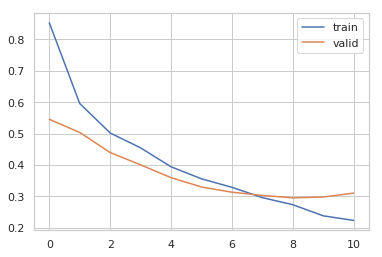
\includegraphics[width=0.5\linewidth]{images/GRU_hl45_REST.png}}
\hfill
\subfloat[\label{b}]{%
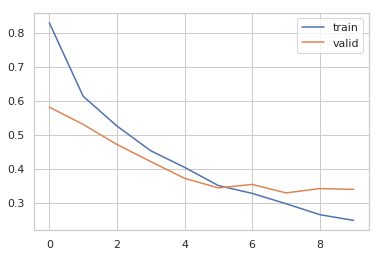
\includegraphics[width=0.5\linewidth]{images/GRU_hl45_LAPT.png}}
\hfill
\subfloat[\label{c}]{%
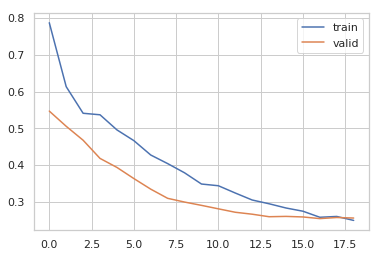
\includegraphics[width=0.5\linewidth]{images/LSTM_hl45_REST.png}}
\hfill
\subfloat[\label{d}]{%
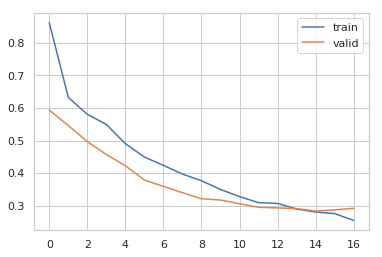
\includegraphics[width=0.5\linewidth]{images/LSTM_hl45_LAPT.png}}
\hfill
\caption{Cross entropy vs. epochs, with 45 number of hidden layers (a) GRU (REST), (b) GRU (LAPT), (c) LSTM (REST), (d) LSTM (LAPT)}
\label{R2} 
\end{figure}

The early stopping procedure saves the duration time for the learning procedure. The training procedure for all the neural network models supposedly has 1000 epochs, yet most of them terminate in the midst of the learning as soon as they overfit. While not using an virtual instance from a cloud computing service, all the neural network training procedures took less than 10 minutes. 

Changing the dropout rate did not really contribute much, surprisingly. One thing our team conjectures is that the effect of dropout might be significant once the training process gets long enough, where it never gets to happen in our case due to the early stopping.

\subsection{Data Representation}

One can remark that using pre-trained word embeddings (namely GloVe for the case of interest) results in a significant gain in terms of efficiency. However, when we restrict our focus on the context where the number of aspects in input is small, bag-of-words representation could still present a decently well constructed model.

One concern is that we might need to depend on neural networks or a more recently developed model in case where one needs to do Aspect-Based Sentimental Analysis with an asymptotic number of possible aspects that a model needs to recognize. In all of the results we have obtained we could remark that for the LAPT dataset (where the number of aspects were close to 100) all of the classical model demonstrate a relatively poor fit. This does not change even when we group of some of the aspects with relatively fewer occurences as $\texttt{OTHER}$. 

\section{Conclusion}

The hypothesis raised in our team's proposal that some classical ML algorithms, such as Logistic Regression, perform well on sparse matrices seems to have some evidence. This is more evident for the REST dataset over the LAPT dataset. Something to note is the surprisingly good performance of Naive Bayes models. 

Among the neural network models, LSTM shows the best fit for both datasets, possibly due to the nature of the reviews where long term dependencies are common. We remark that the test accuracies are in fact better than not only the paper's baselines but also the mentioned best models. LSTM is clearly a worthwhile choice for tasks in natural language processing, particularly aspect-based sentiment analysis. GRU models have been implemented in a very time efficient manner, yet it displays a slightly worse fit. On a concluding note, one should distinguish with care the context when to choose which of two neural network models.

\section{Contribution} 
The authors, Ramsha Ijaz, Aanika Rahman and Dan Yunheum Seol, have all taken direct roles in all classifier implementations, methodology and model evaluations, feature preprocessing, as well as the composition of the report. 

We hereby state that all the work presented in this report is that of the authors.

\bibliographystyle{plain}
\bibliography{report}

\newpage
\onecolumn
\section*{Appendix}

\begin{table}[!htb]
\begin{tabularx}{\textwidth}{@{}l*{5}{C}c@{}}
\toprule
Classifier & Domain (Representation) & Train & Valid & Test \\ 
\midrule
Naive Bayes
& REST (BBoW)      & 84.46 & 85.01 & 79.88 \\
& REST (FBoW)      & 86.94 & 85.15 & 80.76 \\
& REST (TFIDF)     & 86.26 & 84.72 & 83.24 \\
& LAPT (BBoW)          & 84.77 & 79.60 & 69.50 \\
& LAPT (FBoW)          & 86.98 & 82.65 & 71.75 \\
& LAPT (TFIDF)         & 87.02 & 81.59 & 73.87 \\
\midrule
Logistic Regression
& REST (BBoW)      & 88.44 & 89.08 & 79.59 \\
& REST (FBoW)      & 88.39 & 88.65 & 80.47 \\
& REST (TFIDF)     & 92.71 & 93.30 & 81.92 \\
& LAPT (BBoW)          & 94.92 & 91.39 & 70.82 \\
& LAPT (FBoW)          & 96.87 & 93.51 & 69.23 \\
& LAPT (TFIDF)         & 97.04 & 93.91 & 69.23 \\
\midrule
Linear SVM
& REST (BBoW)      & 92.47 & 92.87 & 80.03 \\
& REST (FBoW)      & 94.75 & 95.49 & 78.72 \\
& REST (TFIDF)     & 92.03 & 92.72 & 82.51 \\
& LAPT (BBoW)          & 96.60 & 93.25 & 68.70 \\
& LAPT (FBoW)          & 96.73 & 93.11 & 68.70 \\
& LAPT (TFIDF)         & 93.33 & 90.33 & 72.68 \\
\midrule
Radial SVM
& REST (BBoW)      & 66.88 & 71.62 & 72.89 \\
& REST (FBoW)      & 66.49 & 71.03 & 72.45 \\
& REST (TFIDF)     & 68.87 & 72.20 & 73.47 \\
& LAPT (BBoW)          & 61.32 & 57.75 & 56.76 \\
& LAPT (FBoW)          & 47.51 & 48.08 & 40.98 \\
& LAPT (TFIDF)         & 59.56 & 61.06 & 57.29 \\
\midrule
Decision Trees
& REST (BBoW)      & 74.79 & 80.20 & 73.62 \\
& REST (FBoW)      & 76.69 & 79.48 & 72.89 \\
& REST (TFIDF)     & 75.08 & 76.71 & 73.76 \\
& LAPT (BBoW)          & 75.76 & 77.09 & 66.31 \\
& LAPT (FBoW)          & 76.78 & 79.16 & 62.33 \\
& LAPT (TFIDF)         & 80.00 & 80.93 & 61.14 \\
\midrule
Random Forest
& REST (BBoW)      & 79.94 & 81.95 & 77.26 \\
& REST (FBoW)      & 80.62 & 81.95 & 78.57 \\
& REST (TFIDF)     & 78.34 & 80.20 & 77.55 \\
& LAPT (BBoW)          & 82.30 & 80.53 & 69.23 \\
& LAPT (FBoW)          & 82.30 & 83.31 & 68.70 \\
& LAPT (TFIDF)         & 80.04 & 79.21 & 65.52 \\
\bottomrule
\end{tabularx}
\caption{Train/Valid/Test results for all classifiers using optimum hyperparameters}
\label{A1}
\end{table}

\noindent Graphs for the effect of hyperparameter tuning on simple algorithms can be found in the associated .ipynb file. If interested and unable to find, feel free to contact us. 

\end{document}